\documentclass[onecolumn,12pt]{article}

\usepackage[utf8]{inputenc}
\usepackage[T1]{fontenc}
\usepackage{polski}

\setlength{\voffset}{-0.55in}
\setlength{\headsep}{3pt}

\usepackage{hyperref}
\hypersetup{
    colorlinks=false, %set true if you want colored link
    linktoc=all,     %set to all if you want both sections and subsections linked
}

\usepackage[polish]{babel}
\usepackage{algorithm,algorithmic,lipsum}
\usepackage[utf8]{inputenc}
\usepackage{url}
\usepackage{anyfontsize}
\usepackage{multirow}
\usepackage{subfigure}
\usepackage{tabularx}
\usepackage{ragged2e}
\usepackage{booktabs}
\usepackage{multirow}
\usepackage{grffile}
\usepackage{indentfirst}
\usepackage{caption}
\usepackage{listings}
\usepackage{lipsum}
\usepackage{enumitem}
%\usepackage{xcolor}
%\usepackage{hyperref}
\usepackage{catchfilebetweentags}
\usepackage[smartEllipses]{markdown}
\usepackage[ruled,linesnumbered,lined]{algorithm2e}
\usepackage[bookmarks=false]{hyperref}
\usepackage{mathtools}
\DeclarePairedDelimiter\ceil{\lceil}{\rceil}
\DeclarePairedDelimiter\floor{\lfloor}{\rfloor}

\hypersetup{colorlinks,
    linkcolor=blue,
    citecolor=blue,
    urlcolor=blue}

\usepackage[svgnames]{xcolor}
\usepackage{inconsolata}
\usepackage{fontawesome}

\usepackage{csquotes}
\DeclareQuoteStyle[quotes]{polish}
    {\quotedblbase}
    {\textquotedblright}
    [0.05em]
    {\quotesinglbase}
    {\fixligatures\textquoteright}
\DeclareQuoteAlias[quotes]{polish}{polish}

\usepackage[nottoc]{tocbibind}


\usepackage[
style=numeric,
sorting=nyt,
isbn=false,
doi=true,
url=true,
backref=false,
backrefstyle=none,
maxnames=10,
giveninits=true,
abbreviate=true,
defernumbers=false,
backend=biber]{biblatex}

\lstset{
        %language=Python,  %%  PHP,  C,  Java,  etc.
        basicstyle=\ttfamily\footnotesize,
        backgroundcolor=\color{gray!5},
        commentstyle=\it\color{Green},
        keywordstyle=\color{Red},
        stringstyle=\color{Blue},
        numberstyle=\tiny\color{Black},        
        %  morekeywords={TestKeyword},
        %  mathescape=true,
        escapeinside=`',
        frame=single,  %shadowbox,  
        tabsize=2,
        rulecolor=\color{black!30},
        title=\lstname,
        breaklines=true,
        breakatwhitespace=true,
        framextopmargin=2pt,
        framexbottommargin=2pt,
        extendedchars=false,
        captionpos=b,
        abovecaptionskip=5pt,
        keepspaces=true,                        
        numbers=left,                                        
        numbersep=5pt,                                    
        showspaces=false,                                
        showstringspaces=false,
        showtabs=false,
        tabsize=2
    }

\definecolor{graytext}{gray}{0.6}

\lstdefinestyle{PostgreSQL}{
    literate={ą}{{\k a}}1
    		 {Ą}{{\k A}}1
             {ż}{{\. z}}1
             {Ż}{{\. Z}}1
             {ź}{{\' z}}1
             {Ź}{{\' Z}}1
             {ć}{{\' c}}1
             {Ć}{{\' C}}1
             {ę}{{\k e}}1
             {Ę}{{\k E}}1
             {ó}{{\' o}}1
             {Ó}{{\' O}}1
             {ń}{{\' n}}1
             {Ń}{{\' N}}1
             {ś}{{\' s}}1
             {Ś}{{\' S}}1
             {ł}{{\l}}1
             {Ł}{{\L}}1,
    keywordstyle=\textbf,
}

\SetAlgorithmName{\LangAlgorithm}{\LangAlgorithmRef}{\LangListOfAlgorithms}
\newcommand{\listofalgorithmes}{\tocfile{\listalgorithmcfname}{loa}}

\renewcommand{\lstlistingname}{\LangListing}
\renewcommand\lstlistlistingname{\LangListOfListings}

\renewcommand{\lstlistoflistings}{\begingroup
\tocfile{\lstlistlistingname}{lol}
\endgroup}

\begin{document}
% ----------Strona tytułowa------------
\title{Symulacje procesów ciągłych i algorytmy adaptacyjne\\
Projekt –Symulacja wydobywania ropy}
\author{Magdalena Królikowska, Gabriela Piwar, Sławomir Tenerowicz}
\date{\today}
\maketitle

% ----------Spis treści------------
\tableofcontents
\thispagestyle{empty}

% ----------Raport------------
\section{Wprowadzenie}
 

\section{Cel projektu}
Celem zadania było stworzenie symulacji pożarów, odzwierciedlającej rzeczywiste warunki występujące podczas dużego pożaru, który miał miejsce gdzieś na świecie. W tym celu zmodyfikowaliśmy załączone pliki oil2d.hpp i oil2d.cpp, które poźniej posłużyły do uruchomienia skryptów symulacji w IGA-ADS.  

\section{Opis pożaru}
Pożar, który badaliśmy w ramach naszego projektu, wybuchł \textbf{27 kwietnia 2013 roku w Parku Narodowym Grasslands w Kanadzie}. Ogień pojawił się w pobliżu zachodniej granicy parku i szybko rozprzestrzenił się na wschód przez park, spalając około 1/3 zachodniego bloku. 

\begin{figure}[H]
    \centering
    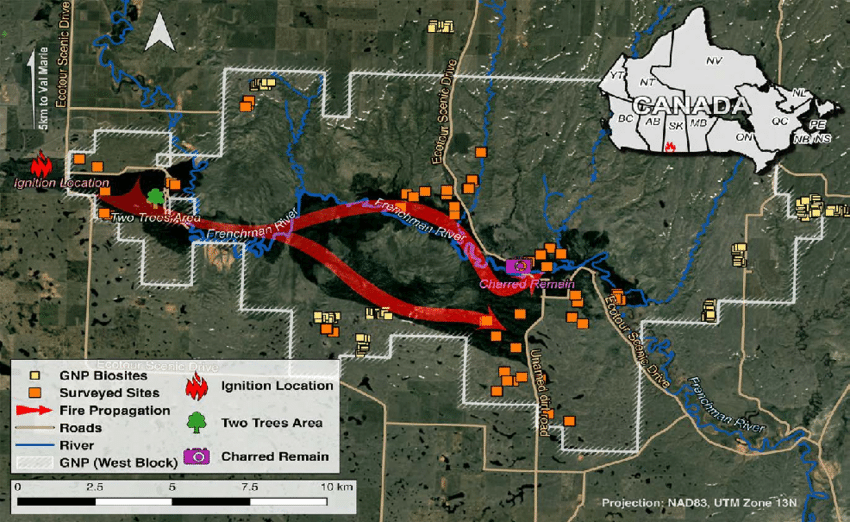
\includegraphics[width=0.9\textwidth]{fire-map-1.png}
    \caption{Grafika złożona ze zdjęć z satelity Landsat 8, wykonanych trzy dni po wybuchu pożaru.}
    \label{fig:example}
\end{figure}
        
\section{Opis rozwiązania}
Tutaj screeny kodu, co zmieniliśmy i jak

\subsection{Modyfikacja wektora wiatru}
Aby odzwierciedlić wpływ zmienności wiatru na rozprzestrzenianie ognia zaimplementowano funkcję custom-wind(x, t). W tym celu w pliku wildfire.hpp  zmieniono funkcję compute-rhs tak, by korzystała z niej do obliczenia wartości bx(x[0], t) i by(x[1], t). Wzór jaki zastosowaliśmy to:
\[
y = 10 \cdot\sin\left(\frac{t}{24} \cdot 2\pi\right) \cdot \sin\left(\frac{x}{100} \cdot 2\pi\right)
\]

\begin{figure}[h]
    \centering
    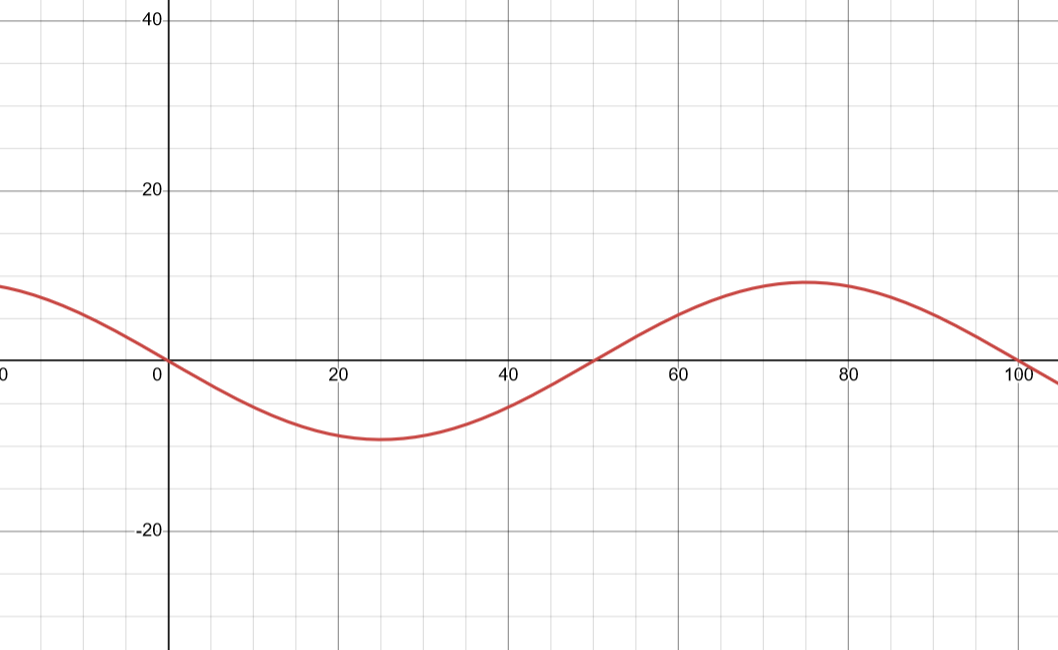
\includegraphics[width=0.9\textwidth]{wind graph.png}
    \caption{Wykres wykorzystanej funkcji.}
    \label{fig:example}
\end{figure}

\begin{figure}[h]
    \centering
    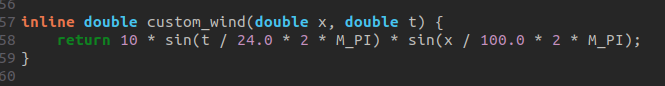
\includegraphics[width=0.9\textwidth]{custom_wind.png}
    \caption{Fragment kodu implementujący funckję wiatru.}
    \label{fig:example}
\end{figure}


\subsection{Początkowa konfiguracja pożaru.}
zmiana punktu rozpoczecia pożaru i promienia, 

\begin{figure}[H]
    \centering
    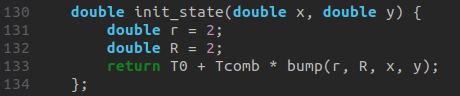
\includegraphics[width=0.9\textwidth]{init_state.png}
    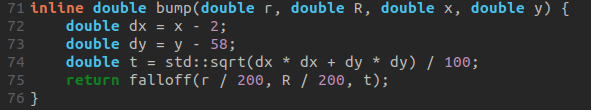
\includegraphics[width=0.9\textwidth]{init_state1.png}
    \caption{Fragment zmienionego kodu dla funkji init_state.}
    \label{fig:example}
\end{figure}

\subsection{Modyfikacja mapy paliwa.}
Mapę mateiałów palnych opracowaliśmy na podstawie zdjęcia satelitarnego. Wydzielając spalony obszar stworzyliśmy maskę binarną, którą przekształciliśmy na macierz 100 x 100. 

\begin{figure}[H]
    \centering
    
\includegraphics[width=0.5\textwidth]{project_wildfire/IMG_0896.png}
    \caption{Wykorzystana mapa paliwa.}
    \label{fig:example}
\end{figure}

W pliku wildfire.hpp dodaliśmy funckję do odczytywania pliku w formacie CSV i przekształcania danych na macierz. Następnie zmodyfikowaliśmy początkowy stan mapy paliwa aby odzwierciedlał dane z pliku.

\begin{figure}[H]
    \centering
    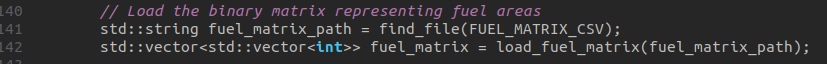
\includegraphics[width=0.8\textwidth]{fuel_map.png}
    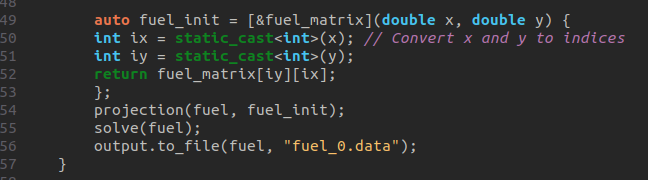
\includegraphics[width=0.8\textwidth]{fuel_map1.png}
    \caption{Fragmenty kodu z implementacji własnej mapy paliwa.}
    \label{fig:example}
\end{figure}

\section{Wyniki}
obrazki jak wyszlo

\section{Podsumowanie}
udalo sie? 


\begin{thebibliography}{9}
\bibitem{texbook}
\href{https://branimirphoto.ca/blog/large-wildfire-burns-through-grasslands-national-park/?fbclid=IwAR10kOfZ03ZdSA12SXVjLDHnmQG8NzV8OXMnwMuYOwZUxyNMMgC7XqHOckw_aem_AbSe3suVXvDvsGvdxdkNPY61Ds63z0wXnrUig_4ZAZlJKoCI8yTPzsxj7_aTuKwY23cInpSUM9UzOpykvzHxRB74}{A large wildfire burns through the Grasslands National Park, Posted by Branimir on 12. May 2013 in Blog / Journal, News & Events}

\bibitem{texbook}
\href{https://www.researchgate.net/figure/The-study-area-is-located-at-the-West-Block-of-Grasslands-National-Park-Canada_fig1_329806684?fbclid=IwAR3PFg0wUu8cTThq5SnfucD4vLfhBDSiHdCm0ItQ_X1MRRAb6wHOB7PSVHk_aem_AbSmS_GuLnzwRWPWYw2-HxWhtIl7nc200yLzsaJgKKWwgPnn3_5GDcWiLcBwMFFKeqdzxou109j5QDsGDAiHqe_6}{Evaluating Post-Fire Vegetation Recovery in North American Mixed Prairie Using Remote Sensing Approaches - Meng Li, Xulin Guo, Department of Geography and Planning, University of Saskatchewan, Saskatoon, Canada}
\end{thebibliography}

\end{document}